\chapter{Optical Detector Applications to measuring the active brain}

The most precise method for measuring brain temperature is to use a thermocouple probe.  The disadvantage of this method and the reason it  can not be used in humans is because it is invasive and damaging.  An optical method would be idea since it is non-invasive and non-damaging.  Currently, there does not exist a method for accurately measuring the temperature of brain tissue optically.  However, other optical measurements methods could be used in conjunction with a temperature model (such as the one proposed here) to calculate the temperature.  The possible application of functional Near-Infrared spectroscopy (fNIRS) and its possible use in brain temperature measurements is discussed along with the limitations of a direct measurement technique such as a thermal imaging camera.
  
\section{{F}unctional {N}ear-{I}nfrared {fNIR} Spectroscopy}
% detector applicaitons to improving fNIR
\begin{figure}[tb]
  \begin{center}
    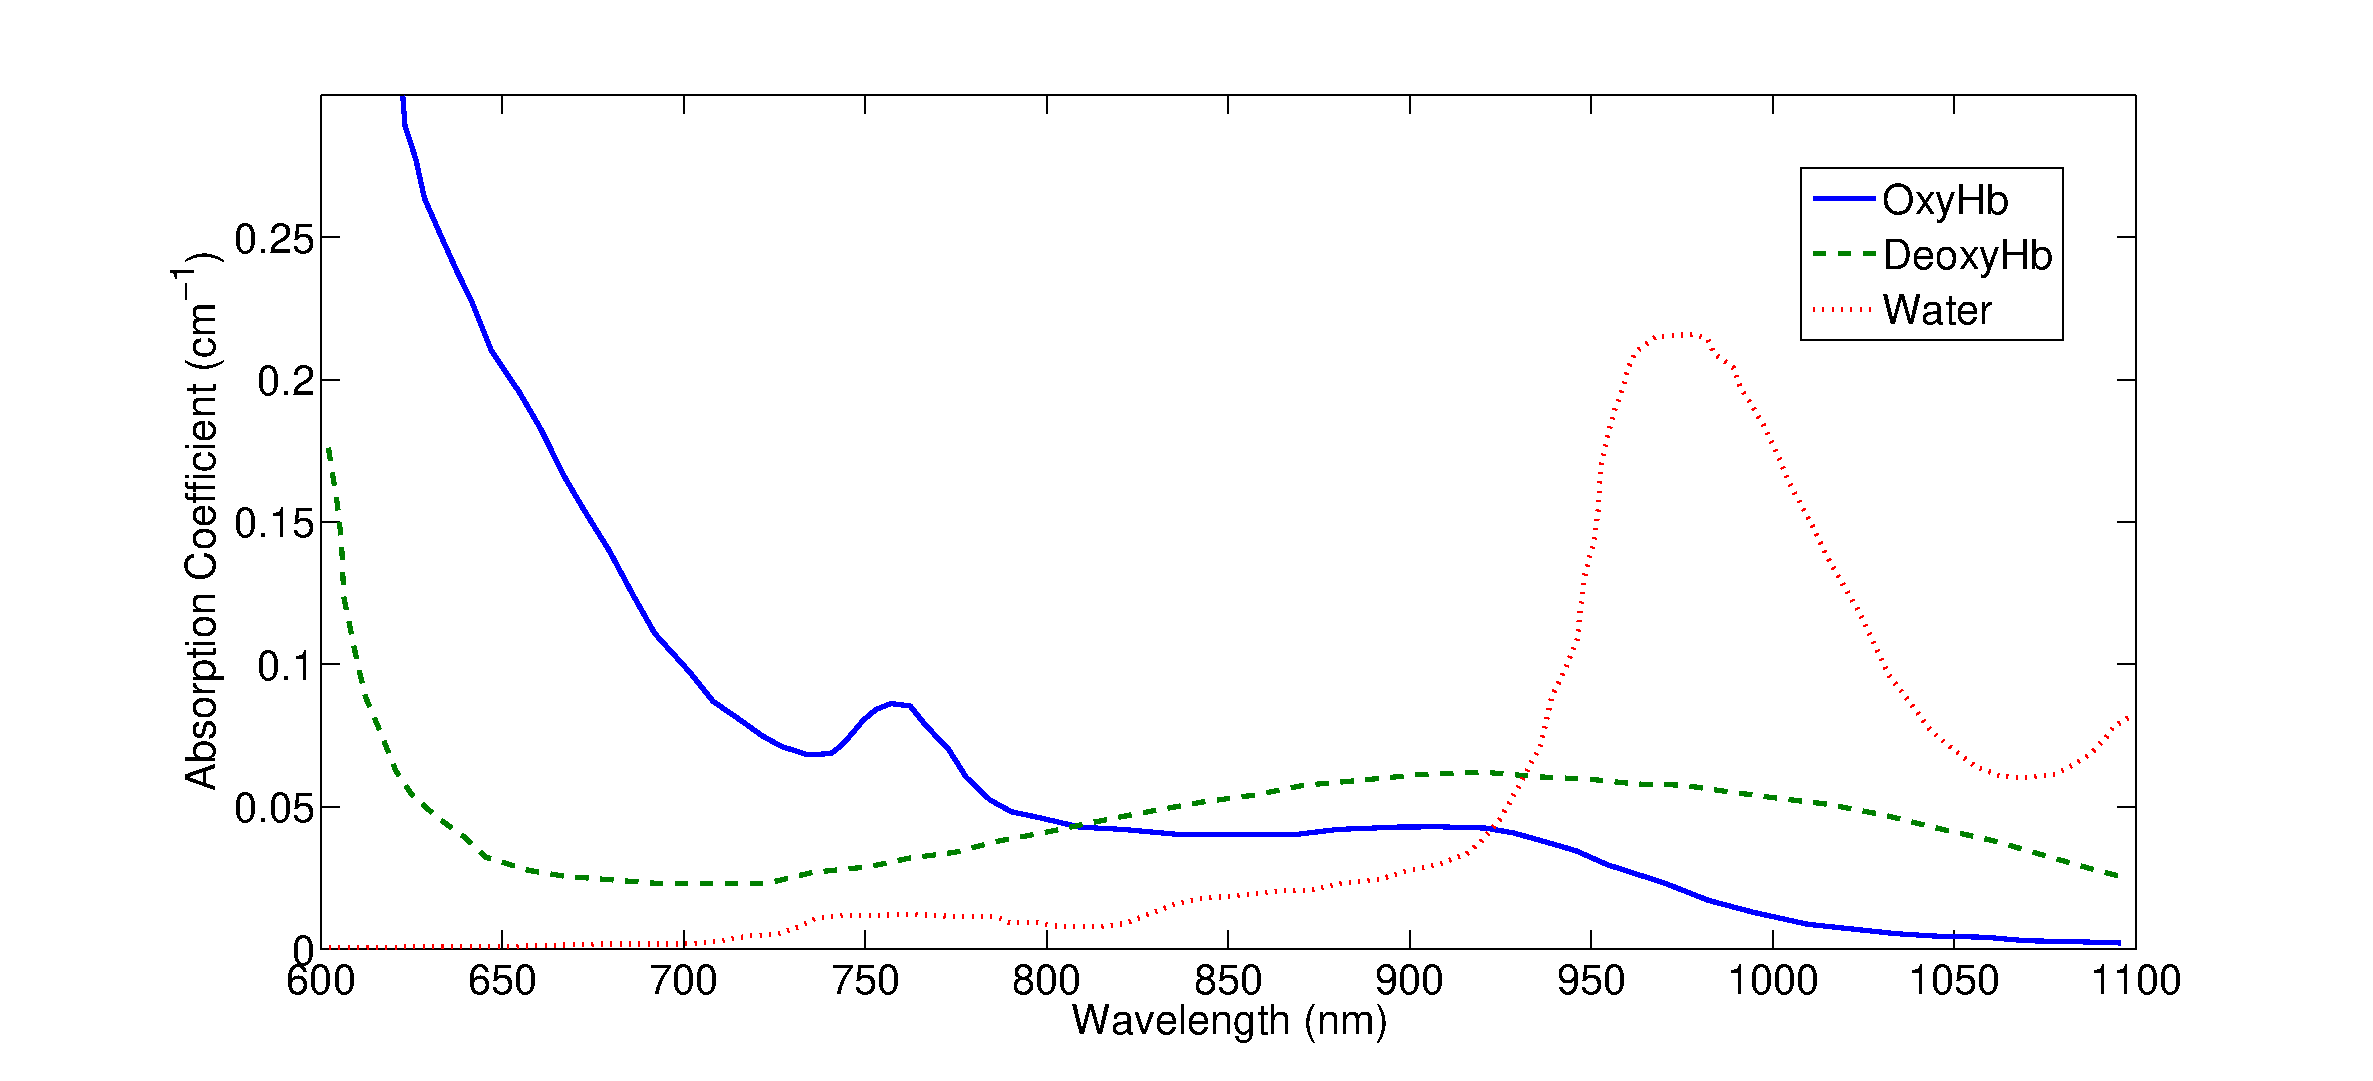
\includegraphics{AbsorptionData}
    \caption[Absorption spectra of water, deoxyhemoglobin and oxyhemoblogin]{\label{fig:fnirabsorption} Absorption spectra of water, Hb and Dhb.  From \citet{cope} and HB stuff from \citet{horecker} }
  \end{center}
\end{figure}

As discussed in previous sections, changes in tissue activity can be detected by measuring the change in blood oxygenation levels.  Functional Magnetic Resonance Imaging (fMRI) is one technique for accomplishing this (through measuring the BOLD response), but other techniques exist.  

The blood oxygenation can be determined by measuring the relative concentrations of oxyhemoglobin (oxy-Hb) and deoxyhemoglobin (deoxy-Hb).  Since oxy-Hb and deoxy-Hb have different absorption spectra (\cref{fig:fnirabsorption}), it is possible to determine this through optical techniques.

\begin{align}
  \label{eq:o2bloodvolume}
  Oxygenation\ &= \Delta C_{HBO2} - \Delta C_{HB} \nonumber \\
  Blood\ Volume\ &= \Delta C_{HBO2} + \Delta C_{HB} 
\end{align}

\section{Temperature Measurements}
\begin{figure}[tb]
  \centering
  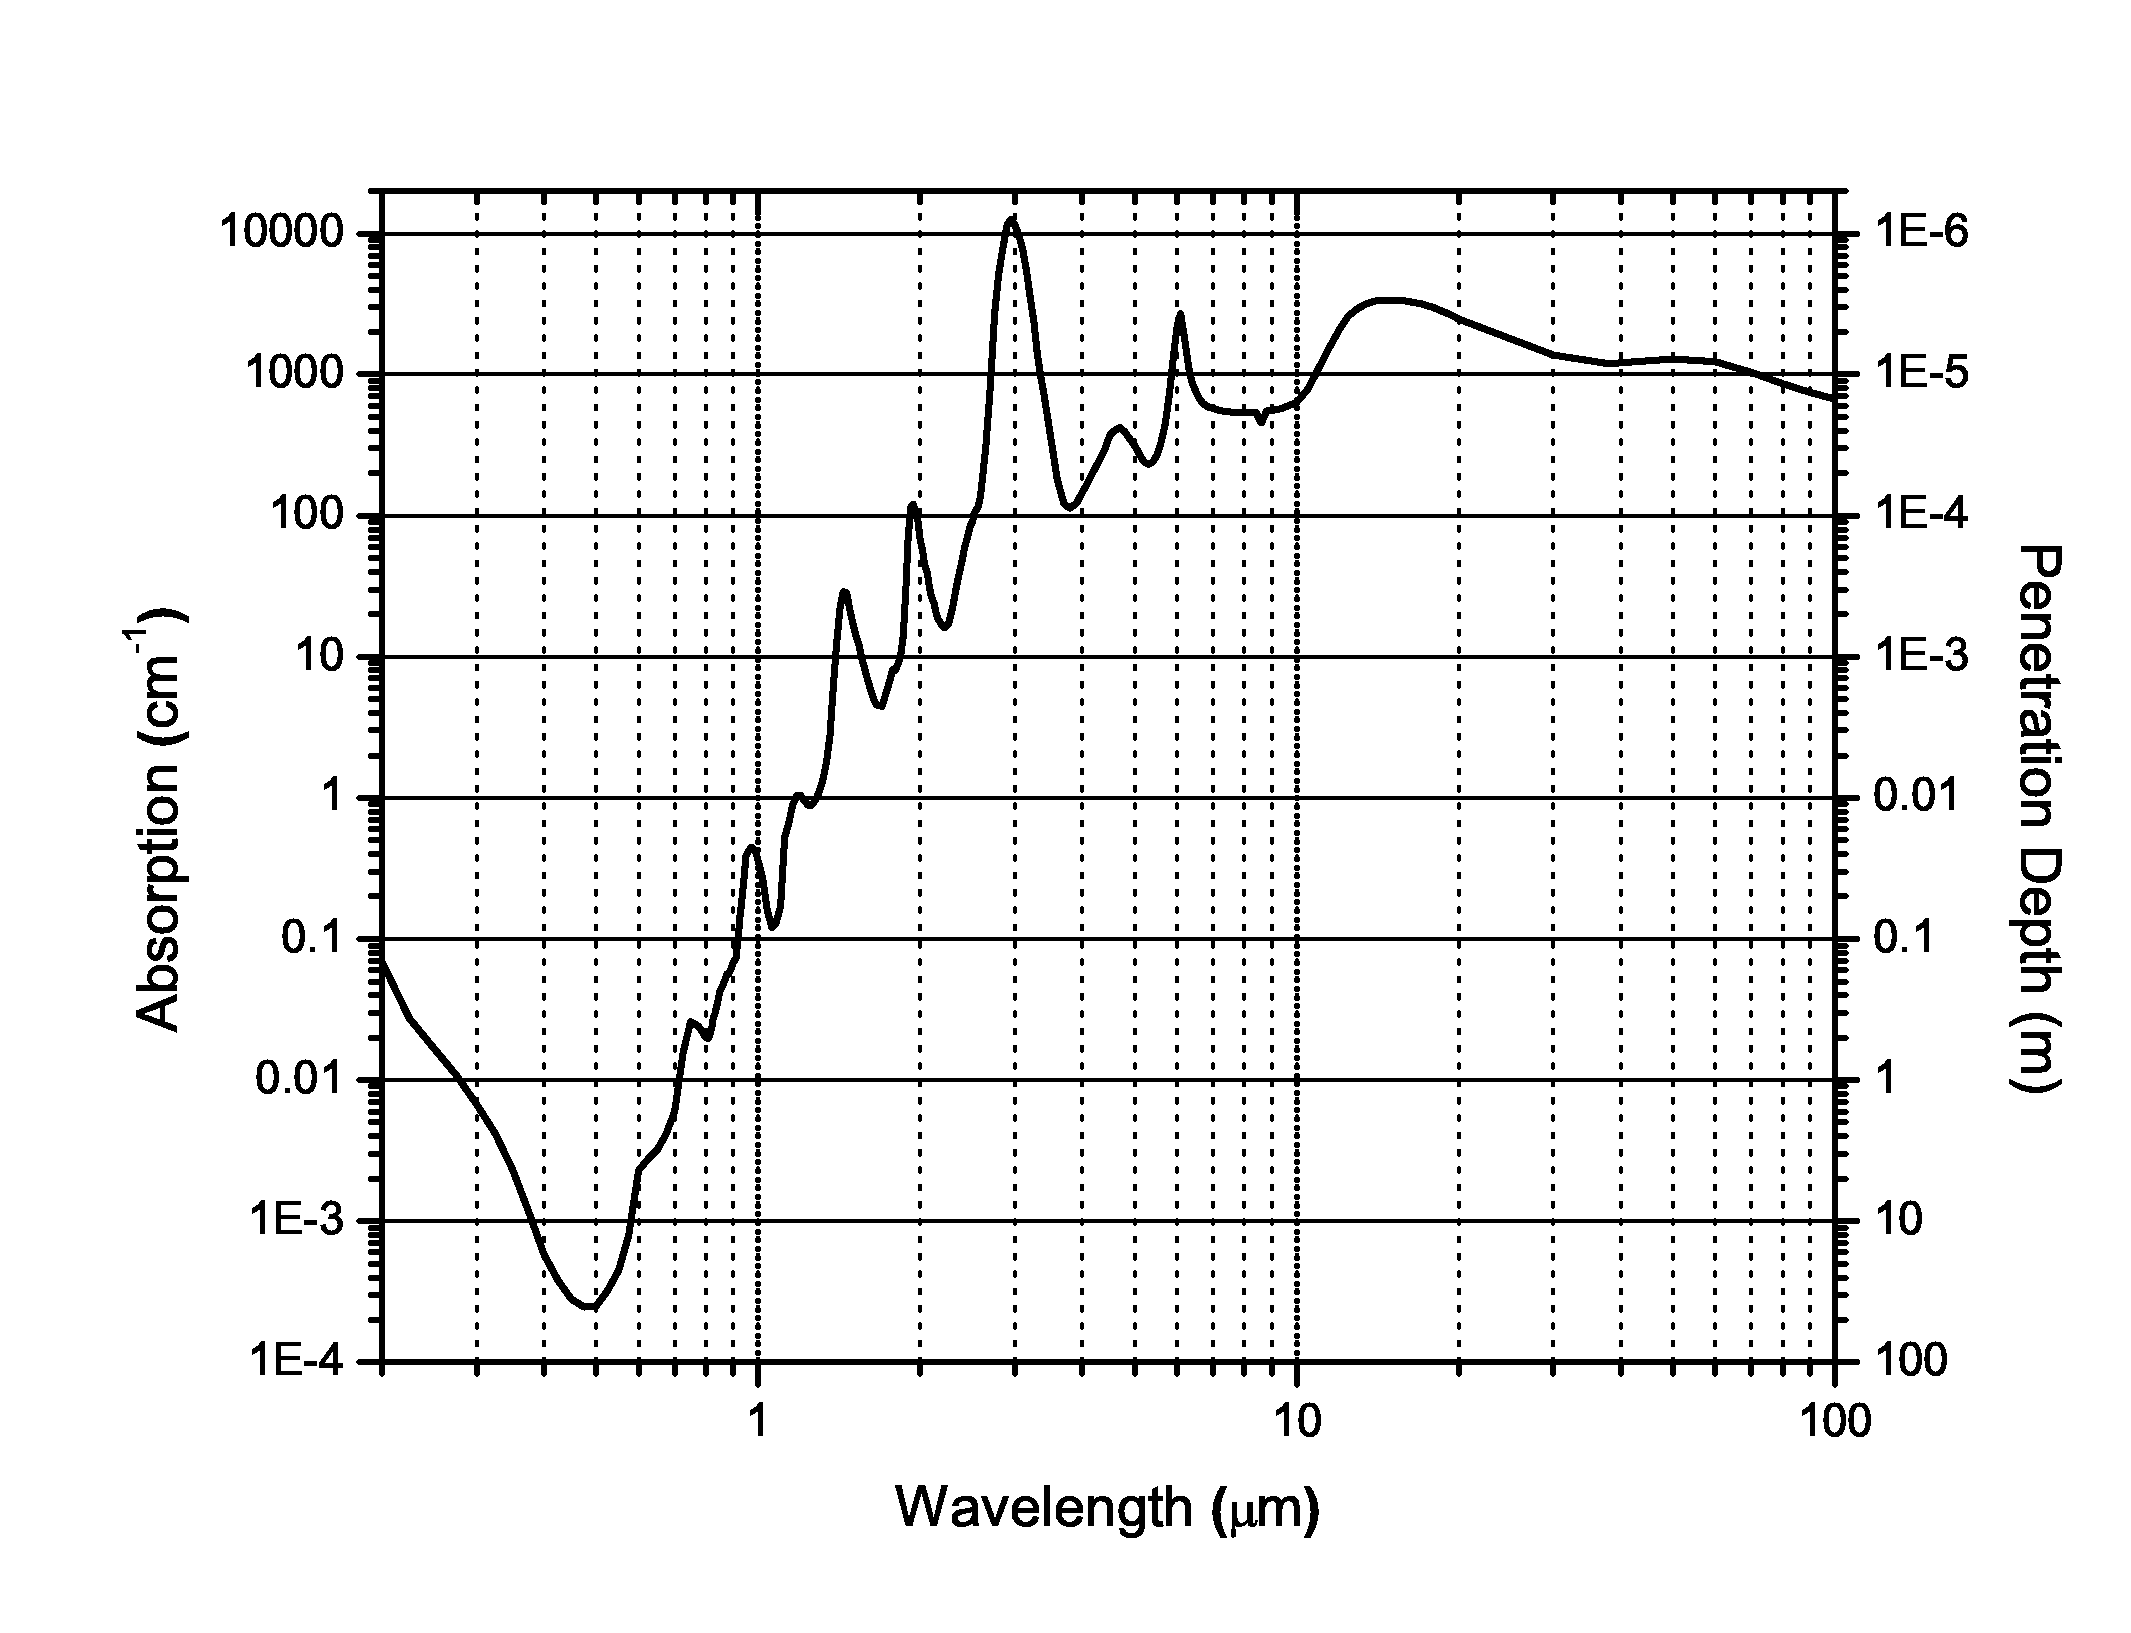
\includegraphics{water-wide-band}
  \caption[Wide-band absorption spectra of water]{\label{fig:waterabs}The absorptions spectra of water from UV to far-infrared.  Modified from~\citet{hale73}.}
\end{figure}

The primary challenge in brain temperature research is making experimental measurements of brain temperature.  The most accurate modality is to use a thermocouple probe, but since this is invasive and causes tissue damage, it is not possible to use this technique with healthy human subjects.  For this reason, a non-invasive technique such as a thermal imaging camera is appealing.  Unfortunately, this technique is limited by the high absorption of infrared photons by water.

Light absorption by a material is modeled using the Beer-Lambert law
\begin{equation}
  I = I_0 e^{-\alpha (\lambda) x} \label{eq:beerlambert}
\end{equation}
where $I$ is the intensity at a depth ($x$) remaining from light with an incident intensity ($I_0$) in a material with absorption coefficient $\alpha$.  The point at which the intensity has decayed to 1/$e$ of the incident intensity is called he penetration depth, $\delta_{p}$
\begin{equation}
  \delta_p = \frac{1}{\alpha (\lambda)} \label{eq:penetrationdepth}
\end{equation}
This equation can be used along with the black body spectrum at tissue temperatures ($37\degree$~C) we can estimate the penetration depth of mid-infrared photons passing through water.

Wien's Displacement Law is a solution to Planck's law for the peak light emission wavelength:
\begin{align}
  \lambda_{max} &= \frac{b}{T} \label{eq:wienslaw} \\
  b &= 2.897 7721 * 10^{-3} \mbox{ K m} \nonumber
\end{align}
where b is Wien's displacement constant and T is the temperature in kelvin.  For $T=300$~K ($T=37\degree$~C), Wien's law yields a peak black-body emission wavelength of 9.66~\textmu m.  

Using~\cref{fig:waterabs} to find the absorption coefficient of approximately 700~cm$^{-1}$.  With the absorption coefficient, the penetration depth (\cref{eq:penetrationdepth}) is approximately 0.14~\textmu m.  This depth is roughly five orders of magnitude smaller than the distance from the surface of the brain to the surface of the head.  Thus, it can be assumed that a thermal imaging camera is unable to image photons coming from the brain.

When a thermal imaging camera is used, the photons collected come from the skin of the head rather than from any deeper tissues, thus it is not a viable form of brain activity detection unless direct line of sight to the brain is available (such as in an open skull surgery).  In this case, the temperature sensitivity of currently available cameras is greater than 14~mK~\citep{flir,ici} so it would be limited to only the most extreme of excitations.  As a comparision, the finger-tapping task discussed in the results section (\cref{sec:experimentalresults}) only induced a peak temperature change of 25~mK after tapping for about 170~seconds.  Detection of this activity would be at the limits of a thermal imaging camera.